% Tamaño de letra.
\documentclass[12pt,titlepage]{report}

%------------------------------ Paquetes ----------------------------------

% Paquetes:

%Para comentarios multilínea.
\usepackage{verbatim}

% Para tener cabecera y pie de página con un estilo personalizado.
\usepackage{fancyhdr}

% Codificación UTF-8
\usepackage[utf8]{inputenc}

% Castellano.
\usepackage[spanish]{babel}

% Tamaño de página y márgenes.
\usepackage[a4paper,headheight=16pt,scale={0.75,0.8},hoffset=0.5cm]{geometry}

% Para poder agregar notas al pie en tablas:
%\usepackage{threeparttable}

% Tipo de letra Helvetica (Arial).
%\usepackage{helvet}
%\renewcommand\familydefault{\sfdefault}

% Gráficos:

% Para incluir imágenes, el siguiente código carga el paquete graphicx
% según se esté generando un archivo dvi o un pdf (con pdflatex).

% Para generar dv.
%\usepackage[dvips]{graphicx}

% Para generar pdf.
\usepackage[pdftex]{graphicx}
\pdfcompresslevel=9

\usepackage{pdfpages}

%
% Directorio donde están las imagenes.
%
%\newcommand{\imgdir}{includes}
%\graphicspath{{\imgdir/}}

%------------------------------ ~paquetes ---------------------------------

%------------------------- Inicio del documento ---------------------------

\begin{document}

% ---------------------- Encabezado y pie de página -----------------------

% Encabezado: sección a la derecha.
% Pie de página: número de página a la derecha.

\pagestyle{fancy}
\renewcommand{\sectionmark}[1]{\markboth{}{\thesection\ \ #1}}
\lhead{}
\chead{}
\rhead{\rightmark}
\lfoot{}
\cfoot{}
\rfoot{\thepage}

% ---------------------- ~Encabezado y pie de página ----------------------

% -------------------------- Título y autor(es) ---------------------------

\title{Información en las organizaciones}
\author{}

% -------------------------- ~Título y autor(es) --------------------------

% ------------------------------- Carátula --------------------------------

\begin{titlepage}

\thispagestyle{empty}

% Logo facultad más pie de la figura.
\begin{center}

\includegraphics[scale=0.55]{./Images/fiuba}\\
\large{\textsc{Universidad de Buenos Aires}}\\
\large{\textsc{Facultad De Ingeniería}}\\
\small{Año 2012 - 1\textsuperscript{er} Cuatrimestre}
\end{center}

\vfill

% Título central.
\begin{center}

\Large{\underline{\textsc{Información en las organizaciones (71.13)}}}

\vfill

% Tabla de integrantes.

\Large{\underline{\textsc{Trabajo Práctico}}}
\vfill

\Large\underline{Ayudante: Licenciada Paez} \linebreak\linebreak
\Large\underline{Integrantes Grupo 2} \linebreak\linebreak

% Separación entre columnas.
\large\addtolength{\tabcolsep}{-3pt}
% Tres columnas con alineación centrada.
\begin{tabular}{|| c | c | c ||}
\hline
\textbf{Apellido, Nombre} & \textbf{Nro. Padrón} & \textbf{E-mail} \\
\hline
Berrilio, Pablo & 88812 & pabloberrilio@gmail.com \\
\hline
Bukaczewski, Verónica & 86954 & vero13@gmail.com \\
\hline
De Antoni, Matías & 88506 & mdeantoni87@gmail.com \\
\hline
Garbarini, Lucía & 88300 & lu.teddy@gmail.com\\
\hline
Invernizzi, Esteban Ignacio & 88817 & invernizzie@gmail.com\\
\hline
Mouso, Nicolás Gastón & 88528 & nicolasgnr@gmail.com \\
\hline
Ygounet, Guido N. & 88246 & gygounet@gmail.com \\
\hline
Zelechowski, Sergio & 86651 & sergiozz123@gmail.com \\
\hline
Moreno Salas, Josué Fabio & Intercambio & josue.nalgarito@gmail.com \\
\hline
\end{tabular}
\end{center}

\vfill

\hrule
\vspace{0.2cm}

% Pie de página de la carátula.
\noindent\small{71.13 - Información en las organizaciones \hfill Grupo 2}

\end{titlepage}

% ------------------------------- ~Carátula -------------------------------

% -------------------------------- Índice ---------------------------------

% Hago que las páginas se comiencen a contar a partir de aquí.
\setcounter{page}{1}

% Índice.
\tableofcontents
\newpage

% -------------------------------- ~Índice --------------------------------

% ----------------------------- Inicio del tp -----------------------------

% Introducción.
%\chapter*{Introducción}
%\addcontentsline{toc}{chapter}{Introducción}

\part{Práctica - Circuitos Te\'oricos}

\chapter{Circuito Pago a Proveedores}
\section{Cursograma Pagos a Proveedores}
\begin{center}
 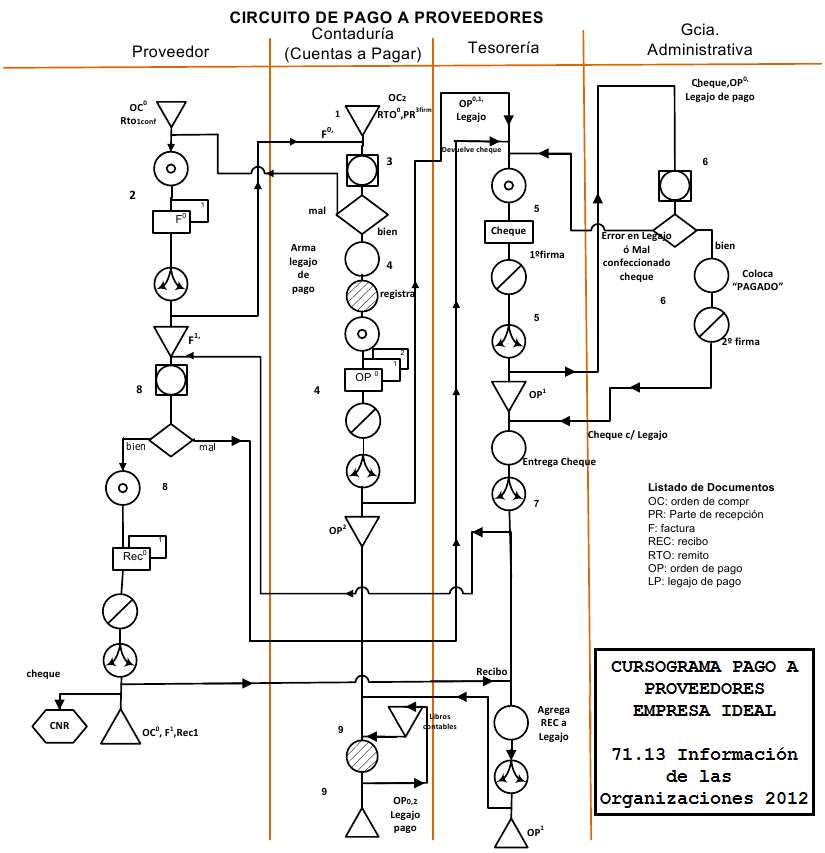
\includegraphics[scale=0.7,keepaspectratio=true]{./Circuitos-Teoricos/Pago-a-Proveedores/Images/cursograma-pago-a-proveedores.png}
 % cursograma-pago-a-proveedores.png: 587x630 pixel, 96dpi, 15.53x16.67 cm, bb=0 0 440 472
\end{center}

\section{Procedimiento de Pagos a Proveedores}
\begin{center}
 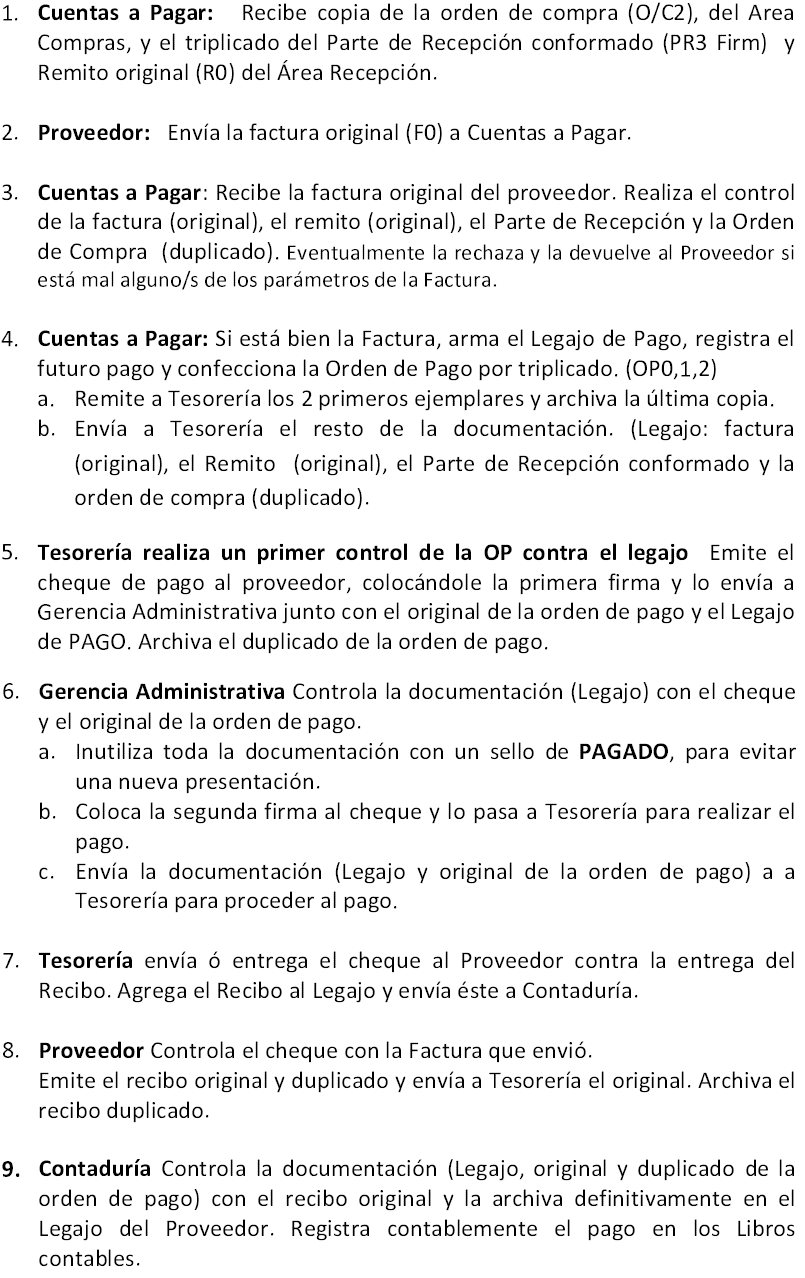
\includegraphics[scale=0.7,keepaspectratio=true]{./Circuitos-Teoricos/Pago-a-Proveedores/Images/procedimiento-pago-a-proveedores.png}
 % procedimiento-pago-a-proveedores-1.png: 805x927 pixel, 96dpi, 21.30x24.52 cm, bb=0 0 604 695
\end{center}

\section{Cursograma de Pagos (con numeración para el manual)}
\subsection{Manual del Cursograma de Pagos}

\begin{center}\textbf{Sectores intervinientes}\end{center}
\begin{itemize}
  \item Proveedor
  \item Contaduría (Cuentas a pagar)
  \item Tesorería
  \item Gcia. Administrativa
\end{itemize}

\begin{center}
  \textbf{Emisión de Documentos}
  
\includegraphics{./Images/Simbolos/simbolo-Emision-de-Documentos.png}
\end{center}
\begin{enumerate}
  \item Proveedor emite factura, original y copia
  \item Proveedor emite recibo del pago, en original y duplicado.
  \item Cuentas a pagar, de acuerdo a la factura recibida, confecciona la Orden de Pago por triplicado.
  \item Tesorería emite cheque de pago a proveedor.
\end{enumerate}

\begin{center}
  \textbf{Documentos}
  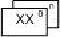
\includegraphics{./Images/Simbolos/simbolo-Documentos.png}
\end{center}
\begin{enumerate}
  \item Factura (F).
  \item Recibo (REC)
  \item Orden de pago (OP).
  \item Cheque
\end{enumerate}

\begin{center}
  \textbf{Distribución}
  
\includegraphics{./Images/Simbolos/simbolo-Distribucion.png}
\end{center}
\begin{enumerate}
  \item Proveedor distribuye factura original a cuentas a pagar, y conserva el duplicado.
  \item Proveedor distribuye recibo original a Tesorería, conserva el duplicado.
  \item Cuentas a Pagar distribuye las órdenes de pago. Original y duplicado a Tesorería, conserva el triplicado.
  \item Tesorería distribuye cheque, orden de pago original y legajo de pago a Gcia. Administrativa.
  \item Tesorería distribuye cheque a proveedor.
  \item Tesorería distribuye  Recibo y Legajo a Contaduría.
\end{enumerate}

\begin{center}
  \textbf{Firma}
  
\includegraphics{./Images/Simbolos/simbolo-Firma.png}
\end{center}
\begin{enumerate}
  \item Proveedor firma recibo.
  \item Cuentas a Pagar firma las órdenes de pago.
  \item Tesorería pone la primera firma en el cheque.
  \item Gcia. administrativa pone la segunda firma en el cheque.
\end{enumerate}

\begin{center}
  \textbf{Almacenamiento Transitorio}
  
\includegraphics{./Images/Simbolos/simbolo-Almacenamiento-Transitorio.png}
\end{center}
\begin{enumerate}
  \item Cuentas a Pagar almacena OC2, RTO0 y PR3firm .
  \item Cuentas a Pagar almacena OP2.
  \item Cuentas a Pagar almacena libros contables.
  \item Tesorería almacena OP1.
\end{enumerate}

\begin{center}
  \textbf{Control y verificación}
  
\includegraphics{./Images/Simbolos/simbolo-Control-y-Verificacion.png}
\end{center}
\begin{enumerate}
  \item Proveedor controla el cheque con la factura que envió, para verificar el cumplimiento del pago de la misma, verificando el monto y el plazo de pago.
  \item Cuentas a Pagar realiza control de factura, remito, parte de recepción y la orden de compra, verificando que la factura haya sido correctamente confeccionada, y que tanto ésta última como el remito y el parte de recepción referencien a la orden de compra en cuestión. 
  \item Gcia. administrativa controla el legajo con el cheque y el original de la orden de pago, verificando que el cheque haya sido correctamente confeccionado, para el proveedor en cuestión y con el monto correcto.
\end{enumerate}

\begin{center}
  \textbf{Decisión}
  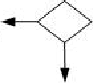
\includegraphics{./Images/Simbolos/simbolo-Decision.png}
\end{center}
\begin{enumerate}
  \item Proveedor controla cheque contra factura, si está bien emite recibo, caso contrario devuelve cheque a Tesorería.
  \item Cuentas a Pagar controla la factura, si está bien confecciona OP, sino la devuelve al proveedor.
  \item Gcia. administrativa controla legajo, OP y cheque, si está bien coloca PAGADO y firma el cheque, caso contrario devuelve la documentación a Tesorería.
\end{enumerate}

\begin{center}
  \textbf{Almacenamiento definitivo}
  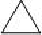
\includegraphics{./Images/Simbolos/simbolo-Almacenamiento-Definitivo.png}
\end{center}
\begin{enumerate}
  \item Proveedor almacena definitivamente OC0, F1 y Rec1
  \item Cuentas a Pagar almacena definitivamente OP0, 2, y Legajo de pago.
  \item Tesorería almacena definitivamente OP1
\end{enumerate}

\begin{center}
  \textbf{Operación}
  
\includegraphics{./Images/Simbolos/simbolo-Operacion.png}
\end{center}
\begin{enumerate}
  \item Cuentas a Pagar arma legajo de pago.
  \item Tesorería entrega cheque.
  \item Tesorería agrega el recibo al legajo de pago.
  \item Gcia. administrativa coloca “Pagado” inutilizando toda la documentación, para evitar nueva presentación.
\end{enumerate}

\begin{center}
  \textbf{Registro}
  
\includegraphics{./Images/Simbolos/simbolo-Registro.png}
\end{center}
\begin{enumerate}
  \item Cuentas a Pagar registra la compra en la cta. cte. proveedores.
  \item Cuentas a Pagar registra contablemente el pago en los libros contables. 
\end{enumerate}

\begin{center}
  \textbf{Circuito no relevado}
  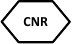
\includegraphics{./Images/Simbolos/simbolo-CNR.png}
  % simbolo-CNR.png: 73x44 pixel, 96dpi, 1.93x1.16 cm, bb=0 0 55 33
\end{center}
\begin{enumerate}
  \item Cobranzas (circuito del proveedor).
\end{enumerate}

\pagebreak
\section{Formularios de Pagos a Proveedores}
\subsection{Orden de Pago} 

\begin{center}
 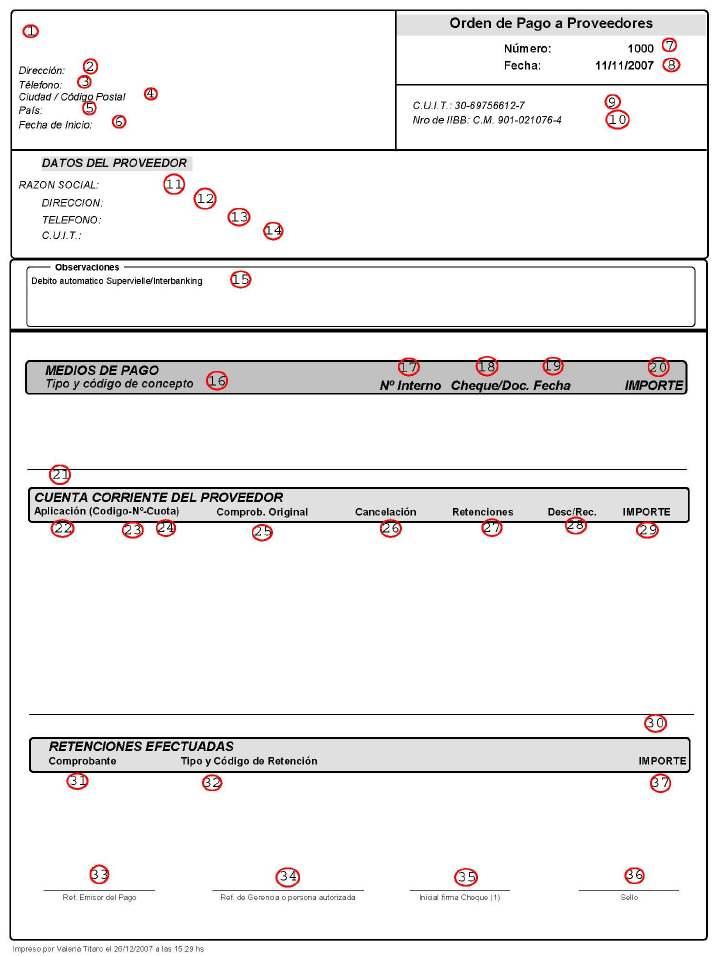
\includegraphics[scale=0.8,keepaspectratio=true]{./Circuitos-Teoricos/Pago-a-Proveedores/Images/orden-de-pago.png}
 % orden-de-pago.png: 721x956 pixel, 96dpi, 19.07x25.29 cm, bb=0 0 541 717
\end{center}

\pagebreak
\begin{itemize}
  \item \textbf{Objetivo:} Con este documento se respalda la emisión del pago que se realizará al proveedor.
Mediante este documento se notifica a los sectores que lo reciben de la existencia y autorización
del pago.
  \item \textbf{Alcance:} Es un documento interno a la empresa.
  \item \textbf{Emisor:} Contaduría.
  \item \textbf{Cantidad de Copias Emitidas:} Original y 2 copias.
  \item \textbf{Sector receptor:} Tesorería.
\end{itemize}

\subsubsection{Descripción}
\begin{center}
 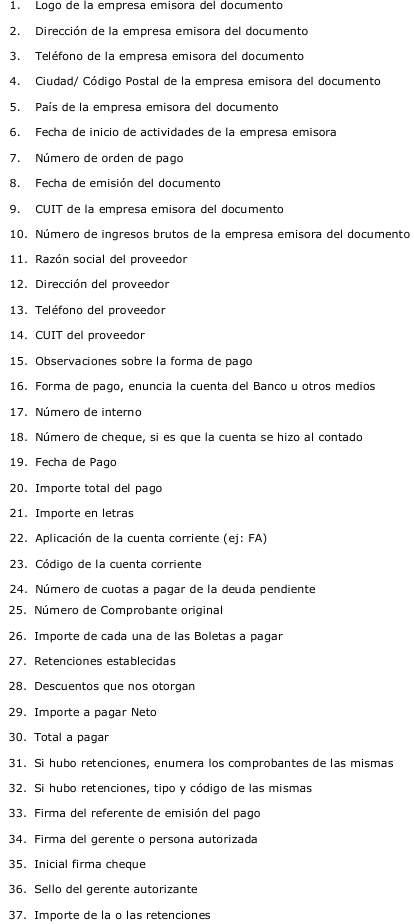
\includegraphics[keepaspectratio=true]{./Circuitos-Teoricos/Pago-a-Proveedores/Images/descripcion-orden-de-pago.png}
 % descripcion-pago-a-proveedores.png: 414x595 pixel, 96dpi, 10.95x15.74 cm, bb=0 0 310 446
\end{center}

\pagebreak
\subsection{Cheque}
\begin{center}
 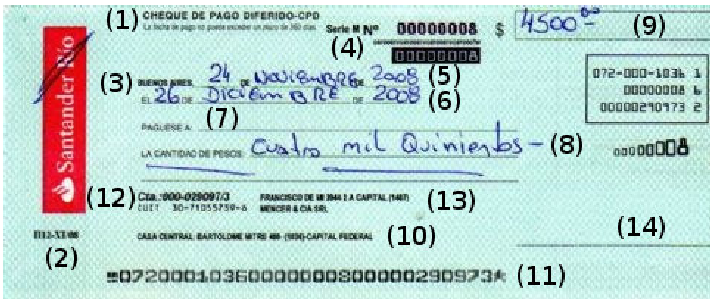
\includegraphics[scale=0.9,keepaspectratio=true]{./Circuitos-Teoricos/Pago-a-Proveedores/Images/cheque.png}
 % cheque.png: 713x304 pixel, 96dpi, 18.86x8.04 cm, bb=0 0 535 228
\end{center}

\begin{itemize}
  \item \textbf{Objetivo:} Con este documento se efectúa el pago. Se entrega al proveedor, y éste por intermedio de un depósito bancario o por ventanilla, obtiene el efectivo que el cheque representa.
  \item \textbf{Alcance:} Es un documento externo a la empresa.
  \item \textbf{Emisor:} Tesorería.
  \item \textbf{Cantidad de Copias Emitidas:} Original.
  \item \textbf{Sector receptor:} Gerencia Administrativa.
\end{itemize}

\subsubsection{Descripción}
\begin{center}
 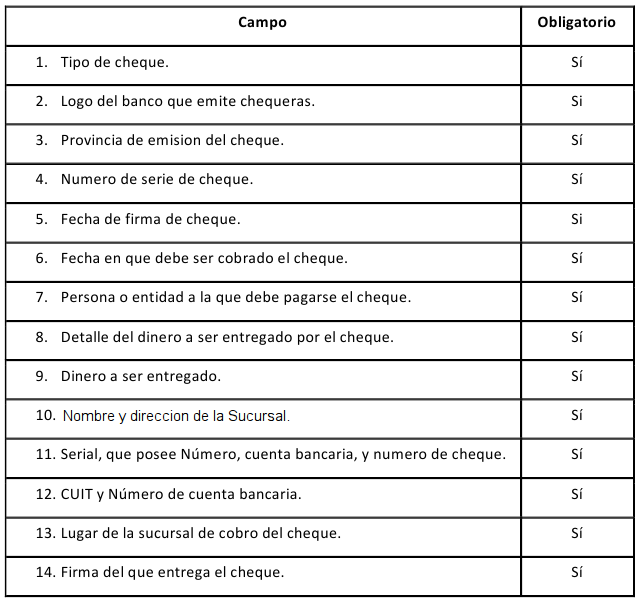
\includegraphics[scale=0.9,keepaspectratio=true]{./Circuitos-Teoricos/Pago-a-Proveedores/Images/descripcion-cheque.png}
 % descripcion-cheque.png: 640x366 pixel, 96dpi, 16.93x9.68 cm, bb=0 0 480 274
\end{center}

\pagebreak
\section{Normas de control interno generales y específicas de Pagos a Proveedores}
\begin{enumerate}
  \item \textbf{Separación de funciones:}
El manejo de los fondos no debe estar a cargo de la misma persona que realiza la registración.  No es conveniente que el cajero realice la registración contable de donde surge el saldo por el cual es responsable, aunque es posible que para su control y para confeccionar las rendiciones que eleva al área contable tenga que efectuar algunas anotaciones.   En el caso particular de los Pagos, la liquidación y autorización debe ser realizada por una persona responsable ajena a Tesorería.
  \item \textbf{Concentración de la responsabilidad:}
Una sola persona será responsable de la custodia y del manejo de fondos, esa persona suele ser el Tesorero.
  \item \textbf{Separación total de los fondos:}
Para un control eficaz de los fondos es recomendable que los provenientes de cobranzas estén separados de los destinados a pagos,  por lo tanto, los valores que tienen origen en las cobranzas se depositaran en su total en la cuenta corriente bancaria y los pagos se efectuaran mediante cheques emitidos contra esa cuenta bancaria.
  \item \textbf{Rotación del personal:}
De manera que se puedan detectar posibles errores en el sistema.  Además, es aconsejable que este personal tome sus vacaciones anuales y que otra persona de la organización esté capacitada para realizar su reemplazo, como así también en casos de enfermedad o egreso del personal.  Los reemplazos se realizaran con personal ajeno al sector y que no tenga amistad o subordinación directa con el reemplazado.
  \item \textbf{Contabilización de las operaciones:}
De manera que permitan el control de las mismas y la consistencia con la información de otros sectores, por ejemplo, total de débitos o créditos en cuentas de terceros.  La registración estará respaldada por la documentación correspondiente.
  \item \textbf{Arqueos sorpresivos:}
Se realizan para verificar si los valores en existencia coinciden con los que surgen de la registración contable.
  \item \textbf{Conciliación bancaria}
\end{enumerate}

\subsection{Normas Específicas}
\begin{itemize}
  \item \textbf{Uso del Cheque:}
  \begin{itemize}
    \item Permite disminuir el riesgo que implica la tenencia de dinero en efectivo.
    \item Ejerce un mejor control sobre los pagos debido a que se podrán conciliar con el resumen bancario.
    \item Deben tomarse en cuenta las distintas modalidades que permite la legislación vigente: Ley 24.452 (Ley de Cheques).
    \item Los cheques deben ser firmados por dos responsables de la organización.
    \item Los cheques que se anulen deben quedar adheridos a la libreta de cheques o destruirse el ángulo inferior derecho donde se firma o en la parte donde figura su numeración.
  \end{itemize}


Con esta forma se persiguen dos finalidades:
  \begin{itemize}
    \item Que exista un control reciproco entre los firmantes y de esta manera detectar errores antes de que el pago se haga efectivo. Esto implica que los dos responsables que firman el cheque efectúen una revisión de la documentación respaldatoria y la inicialicen, puesto que de lo contrario esta norma no tendrá sentido.
    \item Se evita que una sola persona pueda disponer del uso indiscriminado de los fondos, con el consecuente riesgo que ello implica.
  \end{itemize}

  \item \textbf{Pago amparado con la totalidad de los comprobantes y anulación de los mismos:}
En el momento de confeccionar el cheque, la persona responsable tendrá a la vista la
documentación respaldatoria que le da origen y se le colocará el sello de “Pagado” y el
número del cheque con el que se efectúo el pago con el objeto de que no vuelva a ser
presentada para justificar o respaldar otro pago. Quienes firmen el cheque deberán
controlar que se cumpla con estos aspectos.
  \item \textbf{Existencia de fondo fijo o caja chica:}
Tendrá un monto estipulado previamente para realizar los pagos menores en efectivo, estará
a cargo de una persona responsable y su reposición se efectuara periódicamente mediante
la emisión de un cheque previa presentación de los comprobantes que respalden los pagos
efectuados.
  \item \textbf{Pagos de sueldos y jornales:}
Es importante que exista una separación de tareas entre quien controla la asistencia, quien
prepara la liquidación de los haberes y quienes efectúa el pago. En este caso, es de
especial interés la seguridad del movimiento de fondos para el pago (seguros de dinero en
transito, traslado por empresas especializadas, etc.). El pago al empleado se realiza previa
identificación y contra la entrega del recibo firmado.
\end{itemize}


\chapter{Circuito Producci\'on}
\section{Cursograma Producci\'on}
\begin{center}
 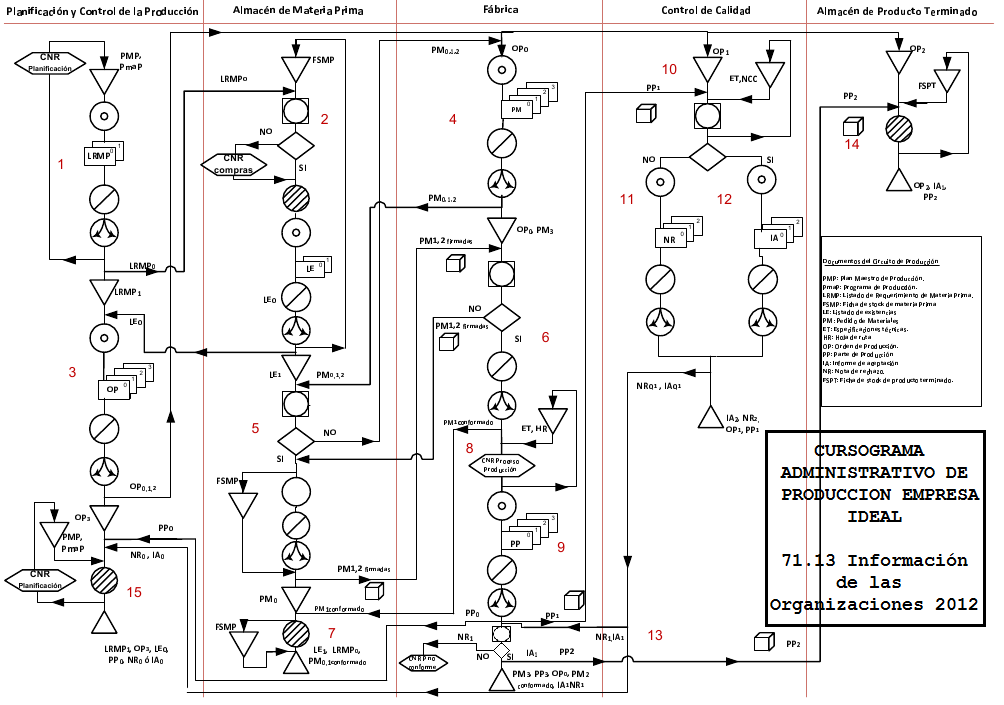
\includegraphics[angle=90,scale=0.95,keepaspectratio=true]{./Circuitos-Teoricos/Produccion/Images/cursograma-produccion.png}
 % cursograma-produccion.png: 1004x705 pixel, 96dpi, 26.56x18.65 cm, bb=0 0 753 529
\end{center}

\section{Procedimiento de Producci\'on}
\begin{center}
 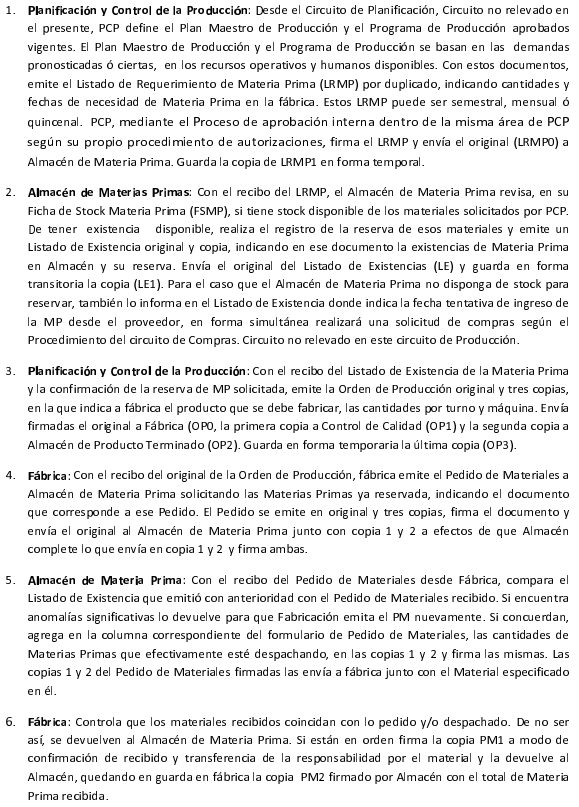
\includegraphics[keepaspectratio=true]{./Circuitos-Teoricos/Produccion/Images/procedimiento-produccion.png}
 % procedimiento-produccion.png: 579x807 pixel, 96dpi, 15.32x21.35 cm, bb=0 0 434 605
\end{center}
\begin{center}
 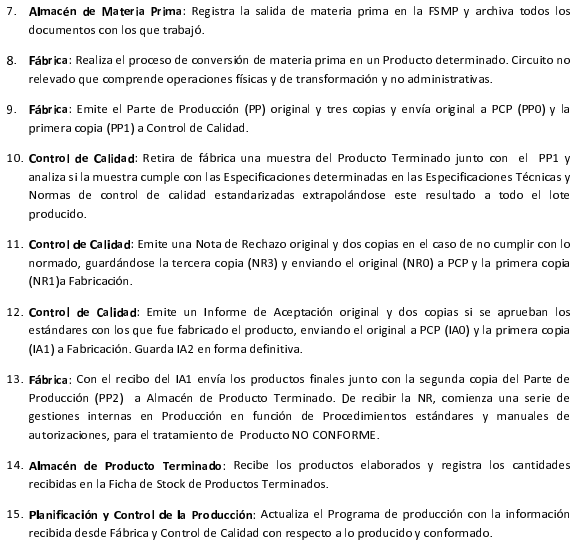
\includegraphics{./Circuitos-Teoricos/Produccion/Images/procedimiento-produccion-2.png}
 % procedimiento-produccion-2.png: 576x545 pixel, 96dpi, 15.24x14.42 cm, bb=0 0 432 409
\end{center}

\pagebreak
\section{Cursograma de Producci\'on (con numeración para el manual)}
\subsection{Manual del Cursograma de Producci\'on}

\begin{center}\textbf{Sectores intervinientes}\end{center}
\begin{itemize}
  \item Planificaci\'on y Control de Producci\'on.
  \item Almac\'en de Materia Prima.
  \item F\'abrica.
  \item Control de Calidad.
  \item Almac\'en de Producto Terminado.
\end{itemize}

\begin{center}
  \textbf{Documentos}
  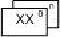
\includegraphics{./Images/Simbolos/simbolo-Documentos.png}
\end{center}
\begin{enumerate}
  \item Listado de Requerimientos de Materia Prima (LRMP).
  \item Orden de Producci\'on (OP).
  \item Listado de Existencia (LE).
  \item Pedido de Materiales (PM).
  \item Parte de Producci\'on (PP).
  \item Nota de Rechazo (NR).
  \item Informe de Aceptaci\'on (IA).
  \item Ficha de Stock de Materia Prima (FSMP).
  \item Ficha de Stock de Producto Terminado (FSPT).
  \item Plan Maestro de Producci\'on (PMP).
  \item Programa de Producci\'on (PmaP).
  \item Especificaciones t\'ecnicas (ET).
  \item Hoja de Ruta (HR).
  \item Normas de Control de Calidad (NCC).
\end{enumerate}

\begin{center}
  \textbf{Emisión de Documentos}
  
\includegraphics{./Images/Simbolos/simbolo-Emision-de-Documentos.png}
\end{center}
\begin{enumerate}
  \item Planificaci\'on y Control de la Producci\'on: emite el LRMP, original y copia.
  \item Planificaci\'on y Control de la Producci\'on: emite la OP, original y tres copias. 
  \item Almac\'en de Materia Prima: emite un LE, original y copia.
  \item F\'abrica: emite el PM, original y tres copias.
  \item F\'abrica: emite el PP, original y tres copias.
  \item Control de Calidad: emite una NR, original y dos copias.
  \item Control de Calidad: emite un IA, original y dos copias.
\end{enumerate}

\begin{center}
  \textbf{Firma}
  
\includegraphics{./Images/Simbolos/simbolo-Firma.png}
\end{center}
\begin{enumerate}
  \item Planificaci\'on y Control de la Producci\'on: se firman las LRMP.
  \item Planificaci\'on y Control de la Producci\'on: se firman las OP.
  \item Almac\'en de Materia Prima: se firman las LE.
  \item Almac\'en de Materia Prima: se firman PM primera y segunda copia.
  \item F\'abrica: se firman los PM.
  \item F\'abrica: se firma la PM primera copia conformada.
  \item F\'abrica: se firman PP.
  \item Control de Calidad: se firman las NR.
  \item Control de Calidad: se firman los IA.
\end{enumerate}

\begin{center}
  \textbf{Distribución}
  
\includegraphics{./Images/Simbolos/simbolo-Distribucion.png}
\end{center}
\begin{enumerate}
  \item Planificaci\'on y Control de la Producci\'on: distribuye LRMP original a Almac\'en de Materia Prima; y converva la copia.
  \item Planificaci\'on y Control de la Producci\'on: distribuye OP original a F\'abrica, la primera copia a Control de Calidad y la segunda copia a Almac\'en de Producto Terminado; conserva la \'ultima copia.
  \item Almac\'en de Materia Prima: distribuye LE original a Planificaci\'on y Control de la Producci\'on; conserva la copia.
  \item Almac\'en de Materia Prima: distribuye PM primera y segunda copia a F\'abrica; conserva el original. \item F\'abrica: distribuye PM original y las dos primeras copias a Almac\'en de Materias Primas; conserva la \'ultima copia.
  \item F\'abrica: distribuye PM primera copia a Almac\'en de Materias Primas. 	
  \item F\'abrica: distribuye PP original a Planificaci\'on y Control de la Producci\'on, la primera copia a Control de Calidad, y la segunda copia a Almac\'en de Producto Terminado; conserva la \'ultima copia.
  \item Control de Calidad: distribuye NR original a Planificaci\'on y Control de la Producci\'on y la primera copia a F\'abrica; conserva la segunda copia.
  \item Control de Calidad: distribuye IA original a Planificaci\'on y Control de la Producci\'on y la primera copia a F\'abrica; conserva la segunda copia.
\end{enumerate}

\begin{center}
  \textbf{Almacenamiento Transitorio}
  
\includegraphics{./Images/Simbolos/simbolo-Almacenamiento-Transitorio.png}
\end{center}
\begin{enumerate}
  \item Planificaci\'on y Control de la Producci\'on: almacena de manera transitoria PMP y PmaP.
  \item Planificaci\'on y Control de la Producci\'on: almacena de manera transitoria LRMP copia.
  \item Planificaci\'on y Control de la Producci\'on: almacena de manera transitoria OP tercera copia.
  \item Planificaci\'on y Control de la Producci\'on: almacena de manera transitoria PMP y PmaP.
  \item Almac\'en de Materia Prima: almacena de manera transitoria FSMP.
  \item Almac\'en de Materia Prima: almacena de manera transitoria LE copia.
  \item Almac\'en de Materia Prima: almacena de manera transitoria FSMP.
  \item Almac\'en de Materia Prima: almacena de manera transitoria PM original.  
  \item Almac\'en de Materia Prima: almacena de manera transitoria FSMP.
  \item F\'abrica: almacena de manera transitoria OP original y PM tercera copia.
  \item F\'abrica: almacena de manera transitoria ET y HR.
  \item Control de Calidad: almacena de manera transitoria OP primera copia.
  \item Control de Calidad: almacena de manera transitoria ET y NCC.
  \item Almac\'en de Producto Terminado: almacena de manera transitoria OP segunda copia.
  \item Almac\'en de Producto Terminado: almacena de manera transitoria FSPT.
\end{enumerate}

\begin{center}
  \textbf{Control y verificación}
  
\includegraphics{./Images/Simbolos/simbolo-Control-y-Verificacion.png}
\end{center}
\begin{enumerate}
  \item Almac\'en de Materia Prima: controla y verifica si tiene stock disponible de los materiales solicitados por Planificaci\'on y Control de la Producci\'on, comparando LRMP recibido y FSMP.
  \item Almac\'en de Materia Prima: controla y verifica si concuerda el pedido de materiales, comparando PM recibido de F\'abrica y el LE emitido anteriormente.
  \item F\'abrica: controla y verifica si los materiales recibidos coincidan con lo pedido y/o despachado.
  \item Control de Calidad: controla y verifica si la muestra del Producto Terminado recibida cumple con las especificaciones determinadas en las ET,
\end{enumerate}

\begin{center}
  \textbf{Decisión}
  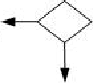
\includegraphics{./Images/Simbolos/simbolo-Decision.png}
\end{center}
\begin{enumerate}
  \item Almac\'en de Materia Prima: Si se tiene el stock disponible se registra la reserva de los materiales y se emite LE; caso contrario se emite LE con una fecha tentativa de ingreso de materia prima desde el proveedor, en forma simult\'anea se realiza una solicitud de compra seg\'un el Procedimiento del circuito de Compras (CNR).
  \item Almac\'en de Materia Prima: Si el PM es correcto entonces se procede a enviar el material; caso contrario lo devuelve a F\'abrica para que emita el PM nuevamente.
  \item F\'abrica: Si los materiales recibidos son los correctos se contin\'ua con la descarga; caso contrario se devuelven los materiales al Almac\'en de Materia Prima.
  \item F\'abrica: Si se recibe el AI se procede al env\'io de los materiales al Almac\'en de Producto Terminado. Si se recibe el NR, se comienza una serie de gestiones internas en funci\'on de Procedimientos est\'andares y manuales de autorizaciones, para el tratamiento de Producto NO CONFORME.
  \item Control de Calidad: Si la muestra pasa los controles de calidad, entonces se procede a emitir el IA; caso contrario se emite una NR.
\end{enumerate}

\begin{center}
  \textbf{Operación}
  
\includegraphics{./Images/Simbolos/simbolo-Operacion.png}
\end{center}
\begin{enumerate}
  \item Almac\'en de Materia Prima: Agrega en la columna correspondiente del formulario PM, la cantidad de materia prima que efectivamente se est\'e despachando.
\end{enumerate}

\begin{center}
  \textbf{Registro}
  
\includegraphics{./Images/Simbolos/simbolo-Registro.png}
\end{center}
\begin{enumerate}
  \item Planificaci\'on y Control de la Producci\'on: registra
  \item Almac\'en de Materia Prima: registra la reserva de materias primas en el LE.
  \item Almac\'en de Materia Prima: registra la salida de materia prima en la FSMP.
  \item Almac\'en de Producto Terminado: registra las cantidades recibidas de productos elaborados en la FSPT.
\end{enumerate}

\begin{center}
  \textbf{Almacenamiento definitivo}
  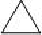
\includegraphics{./Images/Simbolos/simbolo-Almacenamiento-Definitivo.png}
\end{center}
\begin{enumerate}
  \item Planificaci\'on y Control de la Producci\'on: almacena de manera definitiva LRMP copia, OP tercera copia, LE original, PP original y NR original o IA original seg\'un corresponda.
  \item Almac\'en de Materia Prima: almacena de manera definitiva LE copia, LRMP original, PM original y primera copia conformada. 
  \item F\'abrica: almacena de manera definitiva PM tercera copia, PP tercera copia, OP original, PM segunda copia conformada y NR copia o IA copia seg\'un corresponda.
  \item Control de Calidad: almacena de manera definitiva OP primera copia, PP primera copia y IA segunda copia o NR segunda copia seg\'un corresponda.
  \item Almac\'en de Producto Terminado: almacena de manera definitiva OP segunda copia, IA primera copia y PP segunda copia.
\end{enumerate}

\begin{center}
  \textbf{Circuito no relevado}
  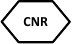
\includegraphics{./Images/Simbolos/simbolo-CNR.png}
  % simbolo-CNR.png: 73x44 pixel, 96dpi, 1.93x1.16 cm, bb=0 0 55 33
\end{center}
\begin{enumerate}
  \item Planificaci\'on y Control de la Producci\'on: Planificaci\'on.
  \item Almac\'en de Materia Prima: Compras.
  \item F\'abrica: Proceso Producci\'on.\
  \item F\'abrica: Tratamiento de Producto NO CONFORME.
\end{enumerate}

\pagebreak
\section{Formularios de Producci\'on}

\subsection{Orden de Producci\'on}
\begin{center}
 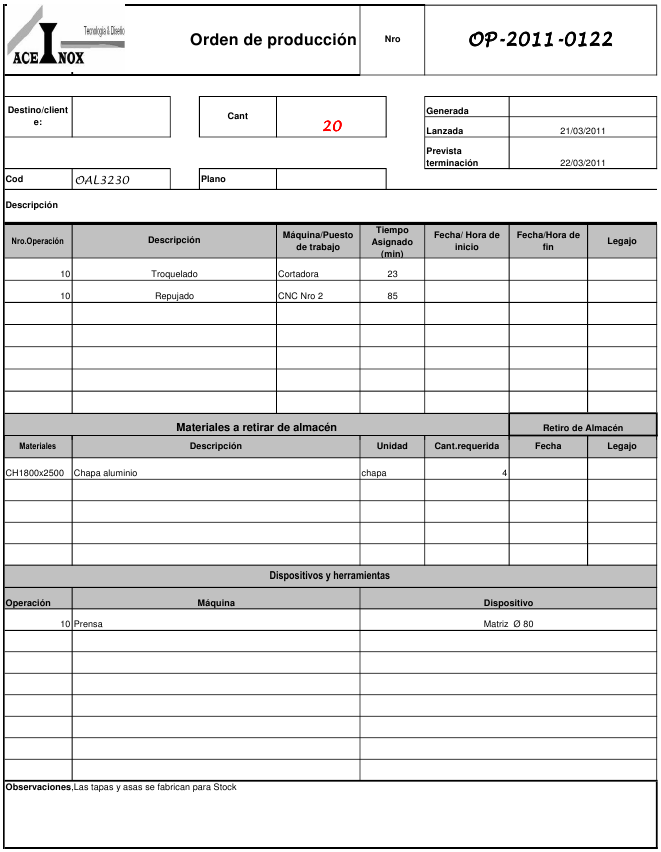
\includegraphics[scale=0.9,keepaspectratio=true]{./Circuitos-Teoricos/Produccion/Images/orden-de-produccion.png}
 % orden-de-produccion.png: 661x852 pixel, 96dpi, 17.49x22.54 cm, bb=0 0 496 639
\end{center}

\pagebreak
\begin{itemize}
 \item \textbf{Objetivo}: Es un documento en el que se especifican las operaciones que deben realizar la producci\'on.
 \item \textbf{Alcance}: Es un documento interno de la empresa.
\end{itemize}

\subsubsection{Descripción}
\begin{enumerate}
 \item Logo de la empresa.
 \item Número de Orden de Producci\'on.
 \item Cliente / Destino.
 \item Cantidad a realizar.
 \item Fecha de generaci\'on de la Orden de Producci\'on.
 \item Fecha de inicio de la producción.
 \item Fecha de finalización de la producción prevista.
 \item N\'umero de código interno de la producci\'on.
 \item N\'umero de plano.
 \item N\'umero de operaci\'on.
 \item Descripci\'on de la operaci\'on.
 \item M\'aquina o puesto de trabajo.
 \item Tiempo asignado (minutos).
 \item Fecha / Hora de inicio.
 \item Fecha / Hora de fin.
 \item N\'umero de legajo.
 \item C\'odigo del material a retirar por almac\'en.
 \item Descripci\'on del material a retirar por almac\'en.
 \item Unidad del material a retirar por almac\'en.
 \item Cantidad requerida del material a retirar por almac\'en.
 \item Fecha de retiro del material del almac\'en.
 \item Legajo de retiro del material del almac\'en.
 \item N\'umero de la operaci\'on donde se utilizar\'a dispositivos y herramientas.
 \item M\'aquina a utilizar.
 \item Dispositivo a utilizar.
 \item Observaciones.
\end{enumerate}

\pagebreak
\subsection{Hoja de Ruta}
\begin{center}
 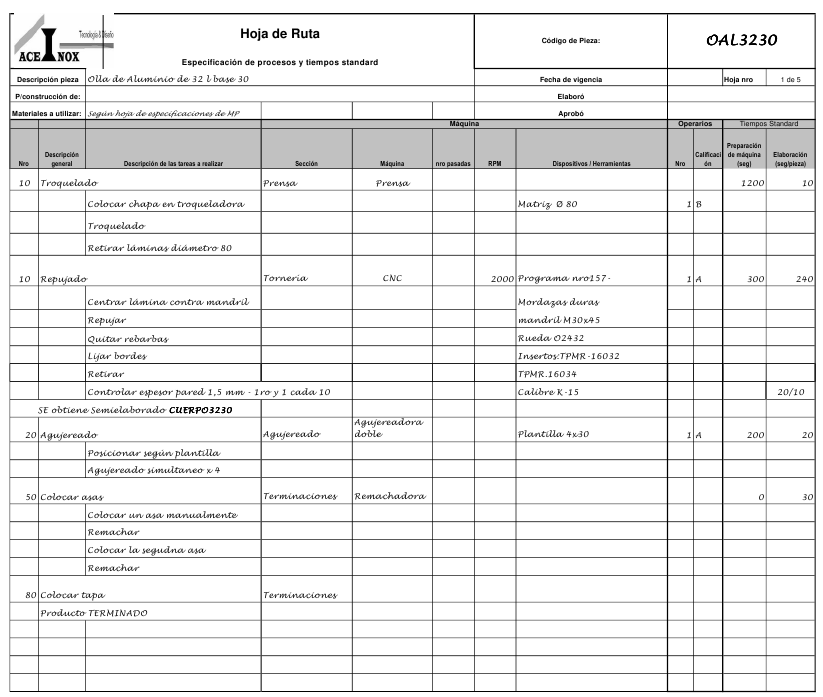
\includegraphics[angle=90,scale=0.95,keepaspectratio=true]{./Circuitos-Teoricos/Produccion/Images/hoja-de-ruta.png}
 % hoja-de-ruta.png: 823x697 pixel, 96dpi, 21.77x18.44 cm, bb=0 0 617 523
\end{center}

\pagebreak
\begin{itemize}
 \item \textbf{Objetivo}: Es un documento en el que se especifican las operaciones que se realizan sobre un mismo artículo hasta el momento de transformarlo en otro.
 \item \textbf{Alcance}: Es un documento interno de la empresa.
\end{itemize}

\subsubsection{Descripción}
\begin{enumerate}
 \item Logo de la empresa.
 \item C\'odigo interno de la pieza.
 \item Fecha de vigencia.
 \item Fecha de elaboraci\'on.
 \item Fecha de aprobaci\'on.
 \item Número de la hoja de ruta.
 \item Descripci\'on de la pieza.
 \item Pedido de construcci\'on.
 \item Materiales a utilizar.
 \item N\'umero de operaci\'on.
 \item Descripci\'on general.
 \item Descripci\'on de las tareas a realizar.
 \item Secci\'on de la m\'aquina. 
 \item Nombre de la m'aquina.
 \item N\'umero de pasadas por la m\'aquina.
 \item N\'umero de revoluciones por minuto para la m\'aquina.
 \item Dispositivos y herramientas.
 \item N\'umero de operario.
 \item Calificaci\'on del operario.
 \item Tiempo standard de preparacion de m\'aquina (segundos).
 \item Tiempo standard de elaboraci\'on (seg/pieza).
\end{enumerate}


\pagebreak
\section{Normas de control interno generales y específicas de Producci\'on}
\begin{itemize}
  \item \textbf{Existencia de inventario permanente o registros contables apropiados:} realización de recuentos físicos periódicos de las existencias, con toma de inventario rotativos, sorpresivos y realizados por personas ajenas a quienes detentan la custodia física de dichos bienes, y de quienes registran los movimientos de los mismos. El inventario físico contribuye a controlar y ajustar los movimientos físicos, evaluar la eficiencia operativa en el manejo de las existencias y sus registraciones, constatar la existencia física y controlar la imputación y valuación contable. Normalmente se debe efectuar un inventario físico total a fin del ejercicio contable.
  \item \textbf{Ajustes de inventario:} Los ajustes por diferencias de inventario deberán estar analizados, justificados y autorizados por un funcionario responsable que sea ajeno a la custodia de los bienes.
  \item \textbf{Custodia de las existencias:} La responsabilidad por la custodia y control de los bienes en existencia, debe recaer sobre una sola persona, a quien se le deben asegurar todas las facilidades de control. El local del depósito debe permitir una protección física adecuada de los bienes.
  Las condiciones del local deben garantizar que no se produzcan deterioros en los productos ( humedad, temperatura, ventilación, etc.)
  \item \textbf{Documentación de todo movimiento de existencias:} Todo movimiento de los bienes en Almacenes, debe estar amparado por el respectivo comprobante, debidamente firmado por un responsable con las atribuciones para realizar los respectivos movimientos.
  \item \textbf{Fijación de puntos de pedido, stocks mínimos y lotes óptimos:} Se recomienda la fijación de stocks de pedido, mínimos, máximos y lotes óptimos de pedido o criterios especiales de reaprovisionamiento.
  \item \textbf{Contratación de seguros adecuados}
\end{itemize}



\part{Análisis de Empresa}
\chapter*{Enunciado}
Enunciado del trabajo práctico...

\chapter{Elección de la empresa}

% TABLA COMPARATIVA
\section{Tabla comparativa de empresas}
\begin{center}
\small\addtolength{\tabcolsep}{-5pt}
\begin{tabular}{|| c || c || c | c | c | c | c ||}
\hline
\hline
T\'{e}rminos & Peso & Empresa 1 & Empresa 2 & Empresa 3 & Empresa 4 & Empresa 5\\
\hline
Contacto   & 10 & 9 & 8 & 10 & 10 & 8 \\
\hline
Ubicaci\'{o}n & 7 & 6 & 10 & 5 & 6 & 7 \\
\hline
Tama\~{n}o & 8 & 9 & 8 & 8 & 3 & 8 \\
\hline
Disp. de info. & 10 & 9 & 6 & 10 & 8 & 8 \\
\hline
Centralizaci\'{o}n & 4 & 8 & 8 & 7 & 6 & 8 \\
\hline
\hline
Totales & - & 326 & 306 & 327 & 270 & 305 \\
\hline
\end{tabular}
\end{center}

%\pagebreak

% ELECCIÓN FINAL.

\section{Elección de la empresa}
Se eligió la empresa \textbf{Empresa X}, principalmente por haber obtenido el mejor puntaje según el criterio de comparación elegido. La buena calidad del contacto y la exelente disponibilidad de información situa a esta empresa por encima de otras propuestas.

\pagebreak


\chapter{Actividad de la empresa IEP De Iluminación}

\begin{center}
 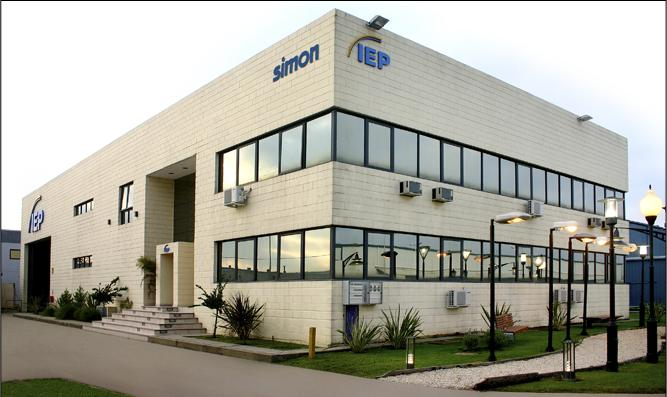
\includegraphics[scale=0.75]{./Images/iep-instalacion.png}
\end{center}

\section{Introducci\'on}
\subsection{Descripción}
Es una empresa multinacional dedicada a la fabricación y comercialización de luminarias, farolas, columnas y soportes, que ofrece soluciones de excelente calidad luminotécnica en Alumbrado Público, Áreas Verdes, Alumbrado Industrial, Alumbrado Interior, Alumbrado de Jardín, Iluminación con Sumergibles y Leds.

\subsection{Ubicación}
La empresa se encuentra ubicada en las afueras de la Ciudad de Buenos Aires, m\'as precisamente en el conurbano bonaerense en el kil\'ometro 37.5 del ramal Escobar de la Ruta Panamericana. A pesar de encontrarse a aproximadamente 
40 kil\'ometros de la Capital Federal, es relativamente f\'acil y r\'apido llegar hasta la f\'abrica.

\subsection{Historia}
En el año 1922 Industrias Electrotécnicas Puig (IEP) se especializaba en la fabricación de aparatos reflectores para alumbrado en la española ciudad de Barcelona.
En el año 1966 pasa a formar parte del Grupo Simon, un holding de empresas del mercado eléctrico español con visionaria expansión hacia a los cinco continentes.
A principios de la década del 90 adapta nuevamente su estructura y su imagen, empezando a conocérsela como IEP DE ILUMINACIÓN.
Es en el año 1998 que IEP DE ILUMINACIÓN llega a la Argentina, convirtiéndose en el lapso de 12 años en la principal responsable de la comercialización de luminarias para toda América del Sur. 
Como en todo proceso de expansión y desarrollo, el Grupo Simon fue incorporando nuevos centros de producción y filiales en Latinoamérica (Argentina, Brasil y México), en Europa (Francia, Reino Unido, Irlanda, Bélgica, Holanda, Noruega, Suiza, Polonia), en África (Marruecos y Egipto) y en Asia (China, India, Rusia, Turquía) para poder llegar con mayor rapidez y eficiencia operativa a todos sus mercados.
En la actualidad cuenta con 24 empresas coordinadas desde su sede central en Barcelona (España) y su presencia mundial alcanza a más de 50 países. Centra sus actividades en el ámbito de la instalación eléctrica con diversas líneas de productos: material eléctrico y protección de circuitos, iluminación, domótica, conexiones para voz y datos, canalizaciones y electrónica. Las más recientes incorporaciones en su línea de negocios comprenden el mobiliario urbano y la seguridad. El primero por su relación con los espacios de iluminación urbana y el segundo porque las innovaciones aplicadas en este campo también incluyen material eléctrico.

\subsubsection{En Argentina}
Durante sus primeros años de actividad en el país, la empresa contó con planta de producción en la localidad de Munro (Buenos Aires) y oficinas comerciales en San Isidro (Buenos Aires), pero el creciente aumento de los volúmenes de venta fundados en la producción de luminarias de avanzada tecnología y diseños de vanguardia, demandó la instalación de una planta fabril de mayor tamaño y capacidad productiva.
Así, posicionada en el ámbito local como la empresa “Líder en Innovación Tecnológica”, IEP DE ILUMINACIÓN cuenta desde el año 2005 con instalaciones propias dentro del Centro Industrial Garín (Buenos Aires), garantizando rapidez operativa y de organización al reunir en un mismo lugar tanto sus áreas Comerciales como las de Producción y Almacenamiento.

\section{Filosof\'ia de la empresa}

\subsection{Misi\'on}

La misi\'on de la empresa consiste en operar un sistema rentable que les permita satisfacer las necesidades actuales y potenciales del mercado luminot\'ecnico, 
ofreciendo productos y servicios con verdadero valor agregado, a fin de construir relaciones fuertes y a largo plazo.

\subsection{Visi\'on}

La empresa define su visi\'on de la siguiente forma:\\
Ser considerada la empresa de iluminaci\'on m\'as pujante convirtiendonos en el proveedor preferido por el mercado luminot\'ecnico al ofrecer los mejores 
productos y servicios del rubro.
 
\section{Estructura de la empresa}

\subsection{Organigrama}
A continuación se presenta el organigrama completo de la empresa. Ver imagen \ref{organigramaIEP}

\begin{figure}[h!]
  \centering
  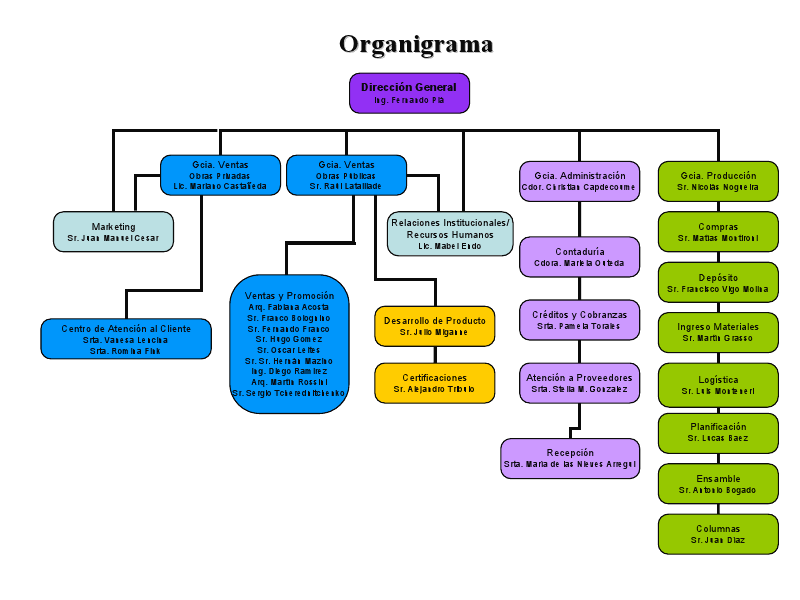
\includegraphics[scale=0.55]{./Images/organigrama.png}
  \caption{Organigrama IEP}\label{organigramaIEP}
\end{figure}

\pagebreak
\section{Circuitos relevados de la empresa}
\subsection{Compra de materiales y entrada de inventario}

\subsubsection{Cursograma}

\subsubsection{Procedimiento}



\subsection{Pedido de ventas con transporte propio}
\begin{enumerate}
\item El cliente solicita un pedido
\item Ventas genera la Solicitud de Pedido de Ventas (SPV) especificando los detalles de la venta ( productos, plazo de entrega tentativo).
	Firma la SPV y envia una copia a comprass???. Archiva temporalmente esta solicitud hasta que concluya el pedido
\item Producci�n recibe la SPV y verifica que cuenta con stock. De no poseer stock necesario se procede a realizar el proceso de Producci�n. 
	En caso de contar con el producto solicitado, se envia "una orden de pedido de productos"
\item Almacen1 recibe la orden de producto ( ya cuenta con el producto, ya sea porque tenia stock o porque lo ha producido especialmente)
	Prepara los productos para su entrega y genera el remito correspondiente. Entrega el producto al Transportista con el original del remito para que sea firmado por el cliente
	Envia otra copia a contaduria.
\item Contaduria genera un listado de remitos sin facturar asociados a esa SPV, y genera la factura correspondiente. Se envia el original de la factura al Transportista para su envio
\item Transportista recibe original y copia del remito y la factura. Envia el pedido junto con la documentacion al cliente.El cliente firma el original del remito y la copia de la factura, y se queda con los otros dos
\item Almacen recibe el original del remito firmado por el cliente y cierra la orden de pedido. 
\item Contaduria recibe la copia de la factura y el remito firmada por el cliente y la asienta como recibida por el cliente. El pago de la factura es parte del sistema de Cobros.
\end{enumerate}
\subsection{Cobro de facturas}

\pagebreak
\section{Presupuesto}

% ------------------------------ Fin del tp -------------------------------

\end{document}

%---------------------------- Fin del documento ---------------------------
